\subsection{Versuchsaufbau}
\label{sec:Versuchsaufbau}
\begin{figure}
  \centering
  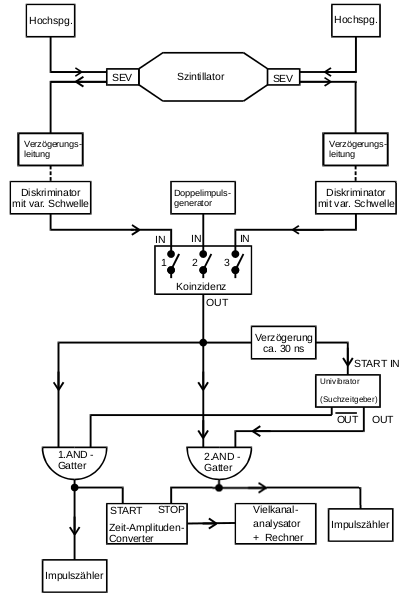
\includegraphics[width=0.9\columnwidth]{pictures/aufbau.png}
  \caption{Blockschaltbild des Versuchsaufbau.\cite{Anleitung}}
  \label{fig:aufbau}
\end{figure}
\subsubsection{Prinzipielle Messmethode}
In Abbildung \ref{fig:aufbau} ist das Blockschaltbild des Versuchsaufbau dargestellt.
Das Szintillatormedium, in welchem die Zerfälle der Myonen detektiert werden, ist organisch und in Toloul gelöst. Es befindet sich in einem Edelstahlzylinder, an dessen Enden jeweils ein Sekundärelektronenvervielfacher (SEV) optisch angekoppelt ist.
Die im Szintillatormedium angeregten Elektronen haben eine Abklingdauer von etwa $\SI{10}{\nano\second}$. Diese liegt also um Größenordnungen unter der Lebensdauer von Myonen (Größenordnung von $\si{\micro\second}$).
Es ist nun die Zeit zwischen dem Auftreten des ersten und zweiten Lichtblitzes, verursacht durch den Eintritt des Myons in den Detektor und durch dessen Zerfall, zu bestimmen.
Da die Zeit zwischen dem Auftreten verschiedener Myonenzerfälle (im Bereich von $\si{ms}$) groß gegen die Myonenlebensdauer ist, kann eine Start-Stop-Schaltung zur Messung der Myonenlebensdauer genutzt werden.
Verwendet wird hierzu ein Zeit-Amplituden-Konverter (TAC). Dieser gibt einen Spannungsimpuls ab, dessen Höhe eine Proportionalität zum zeitlichen Abstand zwischen den beiden Signalen aufweist.
Die durch den TAC generierten Impulse werden entsprechend ihrer Höhe in einen Vielkanalanalysator eingeordnet und gespeichert. Ein Zugriff auf die Daten ist über einen Messrechner möglich.

\subsubsection{Filterung der nicht zerfallenden Myonen}
Wie bereits im Kapitel \ref{sec:Theorie} beschrieben, zerfällt nicht jedes Myon im Szintillator. Über schaltungstechnische Maßnahmen müssen daher alle Myonen, die nur ein Eintrittslichtblitz erzeugen, herausgefiltert werden.
Verwendet wird hierzu eine monostabile Kippstufe, auch bezeichnet als Univibrator. Diese wird über ein Triggersignal in einen instabilen Zustand versetzt und geht nach einer Verzögerungszeit $T_{\mathrm{S}}$ wieder in den stabilen Zustand über.
Genutzt werden kann dies, um eine Suchzeit zu realisieren, in der auf den Eingang eines Zerfallssignals gewartet wird.
Die monostabile Kippstufe wird daher an die beiden SEV über eine Koinzidenzschaltung (näheres hierzu im nächsten Abschnitt) geschaltet.

Tritt nun ein Signal an dem Eingang der monostabilen Kippstufe auf, wird über den $\bar{OUT}$-Ausgang ein $L$-Signal an das 1. AND-Gatter gegeben. Somit wird dieses Gatter inaktiv für ein in der Suchzeit $T_{\mathrm{S}}$ auftretendes weiteres Signal geschaltet. Um trotzdem das START-Signal korrekt weiterzugeben, ist daher darauf zu achten, dass das Signal am Eingang der monostabilen Kippstufe verzögert wird gegenüber dem direkten Signal des Ausgangs der Koinzidenzschaltung welches auf dem zweiten Eingang des 1. AND-Gatters aufgegeben wird.
Das Signal der Koinzidenzschaltung wird ebenso direkt auf das 2. AND-Gatter gegeben, auf welches zudem der $OUT$-Ausgang der monostabilen Kippstufe anliegt. An dem $OUT$-Ausgang liegt während der Suchzeit ein $H$-Signal an.
Nach dem Ende der Suchzeit werden die Signale an den Ausgängen der Kippstufe getauscht.
Tritt nun also ein Startsignal auf, schaltet das 1. AND-Gatter durch und ein Startsignal wird an den TAC gegeben. Durch die Verzögerung vor der Kippstufe schaltet diese anschließend um, sodass ein weiteres Signal innerhalb der Suchzeit als Stopsignal an den TAC gegeben wird.
Tritt kein zweites Signal innerhalb der Suchzeit auf, schaltet die Kippstufe wieder um und die Messung wird verworfen.
Die Suchzeit ist hierbei so zu wählen, dass sie größer als die Lebensdauer der Myonen, aber auch kleiner als die ungefähre Zeit zwischen dem Eintritt zweier verschiedenen Myonen (etwa im Bereich von $\si{\milli\second}$) ist.
Prinzipiell ist der zeitliche Abstand zwischen dem Auftreten verschiedener Myoneneintritte aber statistisch verteilt. Es wird daher in allen Kanälen eine Untergrundrate $U$ gemessen.
An das Signal am START-Eingang des TAC wird zudem ein Zählwerk angeschlossen, um Fehlsignale zu messen.
Ebenso wird an dem STOP-Eingang des TAC ein Zählwerk zur Messung der tatsächlich registrierten Myonzerfälle angeschlossen.
\subsubsection{Unterdrückung von Rauschsignalen}
Einen weiteren Fehler in der Messung stellen spontane, thermische Elektroemissionen an den Photokathoden der SEV dar.
Die so entstehenden Fehlsignale sind aber zumeist kleiner als die durch tatsächliche Myonereignisse erzeugten Signale.
Sie können daher zum Teil bereits über Diskriminatoren herausgefiltert werden.
Die Diskriminatoren geben erst ein Signal weiter, wenn eine gewisse Signalschwelle am Eingang überschritten wird. Zudem sorgen die Diskriminatoren dafür, dass fest definierte logische $H$ und $L$ Spannungssignale an die Schaltung weitergegeben werden. Ein $H$-Signal entspricht hierbei einer Spannung von $\SI{0.8}{\volt}$ und ein $L$-Signal entspricht $\SI{0}{\volt}$.

Um eine noch bessere Rauschunterdrückung zu erreichen, werden zudem die Signale beider SEV auf eine Koinzidenz aufgegeben.
Diese sorgt dafür, dass nur dann ein Signal weitergegeben wird, wenn innerhalb einer Koinzidenzzeit von $\Delta t_{\mathrm{K}}$ von beiden SEV ein Signal registriert wird.
Da die thermische Emission ein statistischer Prozess ist, ist es relativ unwahrscheinlich, dass sie zugleich an beiden SEV auftritt. Bei der Wahl der Koinzidenzzeit ist zu Beachten, dass auch ein Myonzerfall unmittelbar an einem SEV auftreten kann, der zweite SEV das Signal also etwa $\SI{4}{\nano\second}$ später registriert. Zudem haben die SEV verschiedene elektronische Eigenschaften und sind über unterschiedlich lange Kabel angeschlossen.
Diese Effekte können über den Einbau einer zusätzlichen Verzögerungsleitung vermindert werden.
